\documentclass[11pt,a4paper]{article}

\usepackage[utf8]{inputenc}
\usepackage[T1]{fontenc}
\usepackage{lmodern}
\usepackage[margin=2.5cm]{geometry}
\usepackage{microtype}
\usepackage{graphicx}
\usepackage{booktabs}
\usepackage{longtable}
\usepackage{array}
\usepackage{calc}
\usepackage{etoolbox}
\usepackage{xcolor}
\usepackage{enumitem}
\usepackage{caption}
\usepackage[section]{placeins}
\usepackage{fancyhdr}
\usepackage{titlesec}
\usepackage[colorlinks=true,linkcolor=blue!50!black,urlcolor=blue!50!black,citecolor=blue!50!black]{hyperref}
\hypersetup{pdftitle={vNet: a centrally enforced overlay network for on-site programming contests},pdfauthor={Adam Bekkar},
  pdfsubject={Design, implementation and evaluation of vNet, an overlay network for on-site programming contests.},
  pdfkeywords={overlay network, access control, programming contest, TLS, TUN, C++}}

\setlength{\parskip}{0.6em}
\setlength{\parindent}{0pt}
\setlength{\emergencystretch}{2em}
\linespread{1.08}

\titleformat{\section}{\Large\bfseries\sffamily}{\thesection}{0.7em}{}
\titleformat{\subsection}{\large\bfseries\sffamily}{\thesubsection}{0.7em}{}
\titlespacing*{\section}{0pt}{2.2ex plus 0.5ex}{1.2ex}
\titlespacing*{\subsection}{0pt}{1.8ex plus 0.4ex}{0.8ex}

\captionsetup{font=small,labelfont={bf,sf},format=hang,justification=raggedright,singlelinecheck=false,skip=6pt}

\pagestyle{fancy}
\fancyhf{}
\renewcommand{\headrulewidth}{0.3pt}
\fancyhead[L]{\small\sffamily vNet: a centrally enforced overlay network}
\fancyhead[R]{\small\sffamily Adam Bekkar}
\fancyfoot[C]{\small\thepage}
\setlength{\headheight}{14pt}

\renewcommand{\topfraction}{0.9}
\renewcommand{\bottomfraction}{0.8}
\renewcommand{\textfraction}{0.1}
\renewcommand{\floatpagefraction}{0.7}

% Tables, as pandoc writes them: small, with a little room between rows.
\setlength{\LTpre}{0.8em}
\setlength{\LTpost}{0.8em}
\AtBeginEnvironment{longtable}{\small\renewcommand{\arraystretch}{1.25}}
\setkeys{Gin}{width=\linewidth,keepaspectratio}
\providecommand{\tightlist}{\setlength{\itemsep}{0pt}\setlength{\parskip}{0pt}}
\providecommand{\pandocbounded}[1]{#1}
\setlist{nosep}

\title{\sffamily\bfseries vNet: a centrally enforced overlay network for on-site programming contests}
\author{Adam Bekkar\\[0.4em]
\normalsize Former Head of IT at Polympiads (EPFL)\\
\normalsize MSc student in Computer Science at ETH Zurich}
\date{September 2025 to November 2026}

\begin{document}
\maketitle

\begin{abstract}
An on-site programming contest needs a network in which each contestant machine reaches a few organizer services and nothing else, on infrastructure the organizers do not control. vNet is an overlay network built for that case. A conductor admits machines and distributes routes and rules. Switches run by the organizers check every packet against a central access list, reject forged source addresses and cap each machine's rate. An agent on each machine only carries packets.

Every link is mutually authenticated TLS with a role in each certificate. A machine joins through a three-party handshake in which it never names itself to its switch, and a rule change is one edit and one reload on one machine. A host firewall with a configurable bypass contains the machine's physical side.

The implementation is about 6,600 lines of C++17, tested by 135 unit tests and 15 scenarios that run the real programs in network namespaces, including a client that plays the adversary. On a 2-core virtual machine hosting every process, vNet forwards about 650 Mbit/s across two switches with TLS, attaches 400 machines in about 4.2 s and applies a config change for 300 machines in 15 ms. The source and the benchmarks are public at \href{https://github.com/polympiads/vNet}{github.com/polympiads/vNet} and \href{https://github.com/polympiads/vNet-benchmarks}{github.com/polympiads/vNet-benchmarks}, and a deployment test on the EPFL VDI infrastructure is planned for December 2026.
\end{abstract}

\hypertarget{introduction}{%
\section{Introduction}\label{introduction}}

vNet is an overlay network that gives every machine of an on-site programming contest exactly the connectivity the rules allow, and nothing else. Which machine may talk to which is decided on machines the organizers control, never on a contestant's.

\textbf{The event.} Polympiads is the student association that runs mathematics and informatics olympiads at EPFL. The format that motivated vNet is an on-site final: finalists sit in university rooms for one long session, each at a workstation the organizers prepared, and write programs that organizer-run servers build, run and rank. In the format closest to ours, each program is a player for a game designed for that edition, and a game server runs matches between the finalists' players throughout the event.

\textbf{The network this needs.} Each contestant machine must reach a handful of organizer services, such as the game server, a judge and a documentation mirror. It must not reach another contestant's machine, and it must not reach the open internet beyond a short list of addresses. Hosts and runners need wider access, and the rules change while the event runs: a machine is replaced, a service is added, an address is opened for one download.

\textbf{Why this is hard for a student association.} The association does not own the network it runs on. Contestant desktops can be physical machines in one room and virtual desktops from a university VDI pool in another, on subnets and VLANs that only the campus IT service can configure. Isolation therefore cannot rest on switch ports or on a campus firewall. It has to travel with the machines, and it has to be run by a small team of volunteers.

\textbf{Contributions.}

\begin{itemize}
\tightlist
\item
  A design in which no decision that matters is taken on a contestant machine. Switches run by the organizers check every packet against a central access list, reject forged source addresses and cap each machine's rate; the program on the contestant machine only carries packets.
\item
  A control plane a small team can operate under pressure. One roster file generates every key, certificate and config; a rule change is one edit and one reload on one machine; every process recovers from the restart of any other without operator action.
\item
  Containment of the contestant machine's physical side, with the site-specific exceptions (a VDI broker, a DNS server) expressed as configuration instead of code.
\item
  An implementation in C++17 with a test suite that runs the real binaries in Linux network namespaces, including a raw client that speaks the protocol the way an attacker would.
\end{itemize}

\textbf{Context.} I built vNet during my one-year term as Head of IT at Polympiads, as an open-source project under the association's organization. I completed it in autumn 2026, a few months after that term ended, as I began an MSc in Computer Science at ETH Zurich.

\hypertarget{requirements-and-threat-model}{%
\section{Requirements and threat model}\label{requirements-and-threat-model}}

The design follows from seven requirements and from one adversary, the contestant.

\textbf{Requirements.}

\begin{enumerate}
\def\labelenumi{\arabic{enumi}.}
\tightlist
\item
  \emph{Default deny.} A machine reaches only the destinations a rule names.
\item
  \emph{Rules name machines.} A rule says ``contestants may reach the game server'', whatever room, subnet or VDI pool those machines sit in.
\item
  \emph{Enforcement out of reach.} No rule is enforced only by software on the machine it restricts.
\item
  \emph{Live changes.} Adding a machine or a rule during the event restarts nothing and disconnects nobody.
\item
  \emph{Failure of any part.} Any process can crash and restart; contestants who are connected keep working.
\item
  \emph{Operable by volunteers.} One input file, a handful of commands, and a way to see who is missing.
\item
  \emph{Fair sharing.} One machine cannot take the capacity the others need.
\end{enumerate}

\textbf{The adversary.} A contestant has an unprivileged account on their own machine. They can run any program, send any packet into the overlay, and open a TCP connection to anything they can reach on the physical network, including the ports of vNet's own servers. They want to reach another contestant's machine, the open internet or a service the rules do not give them, to pass for another machine, or to disrupt the event.

\textbf{What is trusted.} The organizers' machines (conductor and switches) and the certificate authority key, which is kept off every machine of the overlay. The physical network is trusted to carry packets, not to keep them private: every vNet link is mutually authenticated TLS 1.2 or later.

\begin{longtable}[]{@{}
  >{\raggedright\arraybackslash}p{(\columnwidth - 2\tabcolsep) * \real{0.5000}}
  >{\raggedright\arraybackslash}p{(\columnwidth - 2\tabcolsep) * \real{0.5000}}@{}}
\toprule\noalign{}
\begin{minipage}[b]{\linewidth}\raggedright
\textbf{What the contestant tries}
\end{minipage} & \begin{minipage}[b]{\linewidth}\raggedright
\textbf{What stops it}
\end{minipage} \\
\midrule\noalign{}
\endhead
\bottomrule\noalign{}
\endlastfoot
Send a packet with another machine's source address & The switch compares the source with the address bound to that connection \\
Reach a machine no rule allows & The access list on the sending switch, checked again on the receiving switch \\
Join as another machine & A per-machine key, and a switch that learns the machine's name from the conductor, never from the machine \\
Pose as a switch or as the conductor & The role written in each certificate, checked on every link; two switches also need a token the conductor issued for that pair \\
Inject a route, a token or a config into a switch & Accepted only on the link the switch itself opened to the conductor \\
Exhaust a server with a flood, giant frames or idle sockets & Per-machine rate limits, a 65,994-byte frame bound, a 10 s limit to identify, bounded buffers \\
Go around the overlay through the LAN or IPv6 & A host firewall on the contestant machine (section 6), which holds only while the contestant is not root \\
\end{longtable}

The last row is the weak one and section 6 says so plainly. A contestant who becomes root on their own machine gains nothing inside the overlay, since they hold only their own identity. They do regain the physical network, so a site that can isolate desktops in its infrastructure should do that as well.

\textbf{Out of scope.} Channels that do not use the network (a phone), denial of service against the physical network itself, and compromise of the organizers' machines.

\hypertarget{architecture}{%
\section{Architecture}\label{architecture}}

vNet is three programs: a conductor that decides, switches that enforce and forward, and one agent per machine that only carries packets.

\begin{figure}
\centering
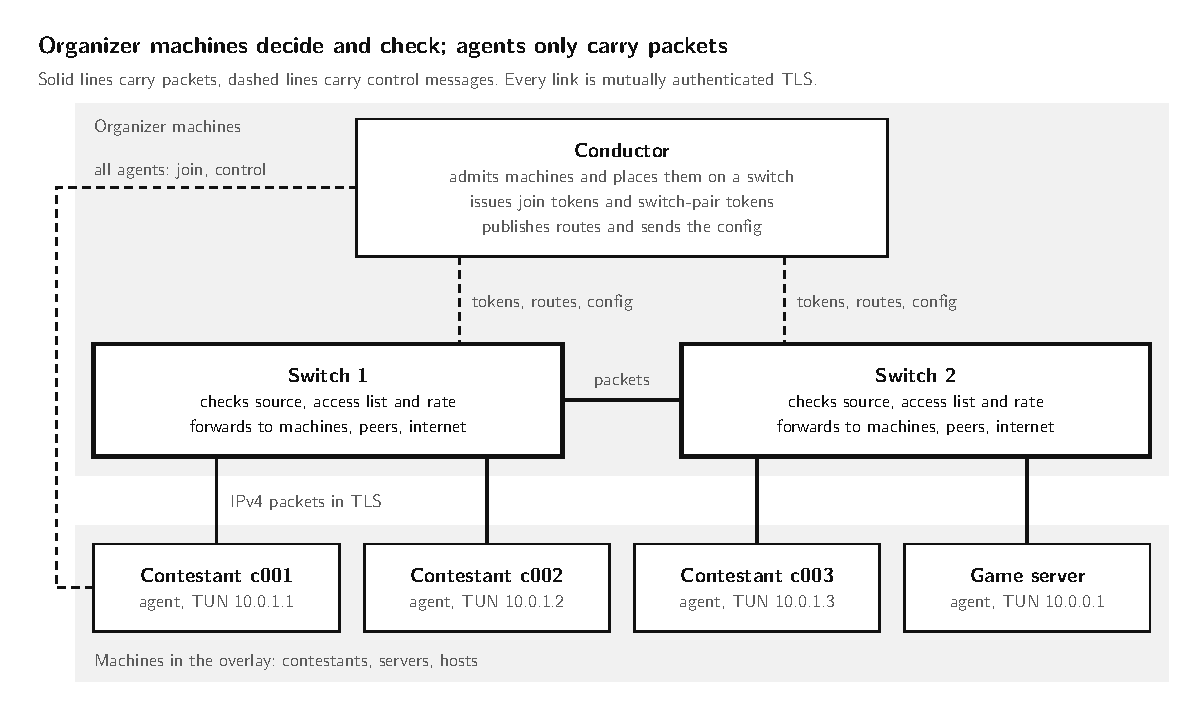
\includegraphics{fig1.pdf}
\caption{Packets travel from agent to switch to switch to agent. The conductor sets that path up and is not on it.}
\end{figure}

\begin{longtable}[]{@{}
  >{\raggedright\arraybackslash}p{(\columnwidth - 6\tabcolsep) * \real{0.1507}}
  >{\raggedright\arraybackslash}p{(\columnwidth - 6\tabcolsep) * \real{0.1644}}
  >{\raggedright\arraybackslash}p{(\columnwidth - 6\tabcolsep) * \real{0.3425}}
  >{\raggedright\arraybackslash}p{(\columnwidth - 6\tabcolsep) * \real{0.3425}}@{}}
\toprule\noalign{}
\begin{minipage}[b]{\linewidth}\raggedright
\textbf{Role}
\end{minipage} & \begin{minipage}[b]{\linewidth}\raggedright
\textbf{Runs on}
\end{minipage} & \begin{minipage}[b]{\linewidth}\raggedright
\textbf{Holds}
\end{minipage} & \begin{minipage}[b]{\linewidth}\raggedright
\textbf{Trusted with}
\end{minipage} \\
\midrule\noalign{}
\endhead
\bottomrule\noalign{}
\endlastfoot
Conductor & One organizer machine & The list of machines and keys, the switch config, the map of who is where & Admitting machines, placing them on switches, issuing tokens, distributing routes and the config. It never forwards a packet. \\
Switch & One or more organizer machines & The access list, the routes, one connection per local machine & Every per-packet decision: source check, access list, rate limit, forwarding to a local machine, a peer switch or the internet. \\
Agent & Every machine in the overlay & Its own key and certificate, nothing about other machines & Nothing. It reads packets from a TUN interface and hands them to its switch, and back. \\
\end{longtable}

\textbf{A separate control plane.} The conductor is not on the data path. Once two machines have joined, their packets travel agent to switch to switch to agent, and keep doing so while the conductor is down. What stops without it is joining.

\textbf{Several switches.} A switch is a single-threaded process, so capacity is added by adding switches. The conductor places each joining machine on a switch its network can reach, round-robin, and moves the machine to another switch when its own dies.

\textbf{Addresses.} Each machine gets one virtual IPv4 address, fixed by the config, inside an overlay prefix (10.0.0.0/8 unless set otherwise). The agent puts that address on a TUN interface as a /32. Applications use it like any other interface and need no change.

\textbf{One transport.} Every link is a TCP connection wrapped in TLS, with a certificate on both ends. A single transport keeps the implementation small, with one event loop, one framing and one TLS library; section 10 discusses what it costs.

\hypertarget{control-plane}{%
\section{Control plane}\label{control-plane}}

The control plane answers four questions: who a connection is, where a machine should attach, how switches learn about each other, and what happens when something dies.

\hypertarget{identity}{%
\subsection{Identity}\label{identity}}

A machine proves who it is with two independent things. The first is a random key, listed with its name and role in the conductor's auth file and compared in constant time. The second is a certificate signed by the event's certificate authority, whose subject carries the role: \texttt{conductor}, \texttt{switch} or \texttt{agent}. Each side of every link checks the role of the other, so the files on a contestant machine cannot be used to run a switch or a conductor. Host names are not checked, because contest machines have no stable names; the role is what matters.

\hypertarget{joining}{%
\subsection{Joining}\label{joining}}

A machine joins in a three-party handshake in which it never tells the switch its own name.

\begin{figure}
\centering
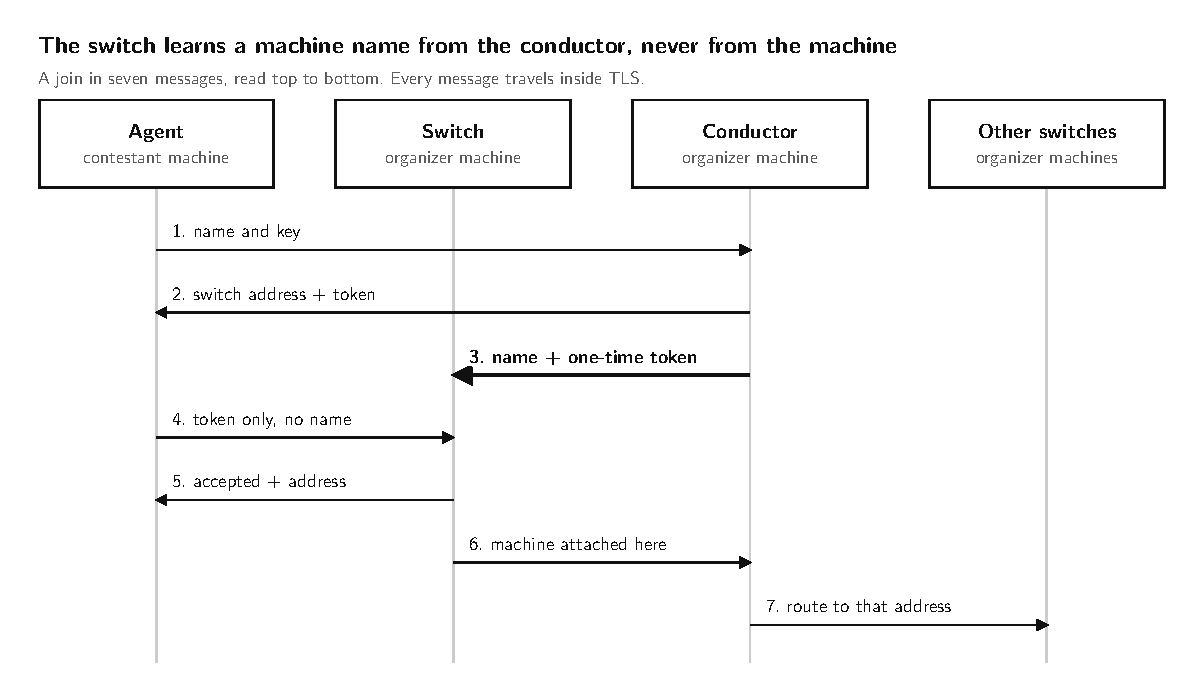
\includegraphics{fig2.pdf}
\caption{The conductor hands the same token to the machine and to the switch (messages 2 and 3). The machine shows it to the switch (4), which answers with the machine's virtual address (5).}
\end{figure}

The token is 64 bits from a cryptographic random generator, valid once and for 60 seconds. The switch receives it from the conductor together with the machine's name, so the name a switch binds to a connection is the one the conductor authenticated. The virtual address comes from the config for that name. A machine cannot ask for an address, and it cannot present a token issued to another machine without having stolen it from a TLS link.

If a machine joins while an older connection under the same name still exists (a frozen VM, a link that died silently), the newer connection wins on both the conductor and the switch.

\hypertarget{routes-and-switch-to-switch-links}{%
\subsection{Routes and switch-to-switch links}\label{routes-and-switch-to-switch-links}}

When a switch accepts a machine it tells the conductor, which publishes the route (virtual address, switch name, switch address) to every other switch. Switches open links to each other on demand, when a route first points to a peer. The conductor issues a fresh token for every pair of switches; whichever side dials presents it, so a process with a stolen switch certificate still cannot attach to the mesh without the conductor's consent. A packet that arrives before its route is held for up to 5 seconds, at most 16 packets per destination, then dropped.

\hypertarget{distributing-the-config}{%
\subsection{Distributing the config}\label{distributing-the-config}}

The switch config, which assigns addresses and lists the allowed pairs, lives in one file on the conductor. The conductor sends it to each switch as it registers and to all of them after a reload signal. A file larger than one frame travels in pieces of at most 60,000 bytes; the switch parses the whole only when the last piece has arrived, and applies it without touching connected machines. Each switch answers with a SHA-256 fingerprint of the parsed content in a canonical order, so the conductor's log shows which switch runs which rules, independent of comments or line order. A switch that has not received a config yet accepts no machine.

\hypertarget{liveness-and-recovery}{%
\subsection{Liveness and recovery}\label{liveness-and-recovery}}

Every link carries heartbeats (10 s by default) and is declared dead after 30 s of silence. No recovery path needs an operator.

\begin{longtable}[]{@{}
  >{\raggedright\arraybackslash}p{(\columnwidth - 4\tabcolsep) * \real{0.2329}}
  >{\raggedright\arraybackslash}p{(\columnwidth - 4\tabcolsep) * \real{0.3836}}
  >{\raggedright\arraybackslash}p{(\columnwidth - 4\tabcolsep) * \real{0.3836}}@{}}
\toprule\noalign{}
\begin{minipage}[b]{\linewidth}\raggedright
\textbf{Failure}
\end{minipage} & \begin{minipage}[b]{\linewidth}\raggedright
\textbf{Traffic meanwhile}
\end{minipage} & \begin{minipage}[b]{\linewidth}\raggedright
\textbf{Recovery}
\end{minipage} \\
\midrule\noalign{}
\endhead
\bottomrule\noalign{}
\endlastfoot
The conductor restarts & Joined machines keep talking; nothing new can join & Switches redial every 2 s and announce the machines they hold; agents reattach their control connection \\
A switch dies & Its machines are cut off & Their agents ask the conductor for another switch and keep their TUN interface and address; routes are withdrawn, then published again \\
The conductor link of a switch is cut & It keeps serving its own machines; after 30 s of silence the conductor withdraws its routes from the other switches & It redials every 2 s and announces its machines again, which republishes the routes \\
An agent is killed & That machine only & Its service restarts it; the new agent restores the physical default route the dead one left diverted \\
One identity appears twice & The older connection is closed & None needed \\
\end{longtable}

\hypertarget{data-plane}{%
\section{Data plane}\label{data-plane}}

A packet from one contestant machine to a server crosses four user-space processes (agent, switch, switch, agent) and is checked on both switches.

\hypertarget{framing}{%
\subsection{Framing}\label{framing}}

Every message on every link starts with a 6-byte header: a 32-bit payload length and a 16-bit type, big endian. Control messages are Protocol Buffers. Data is the raw IPv4 datagram as it was read from the TUN interface, with no wrapper, so forwarding a packet costs no serialization. The protocol has 17 message types whose numbers are fixed for the life of the protocol; a removed type's number is not reused. A header that announces more than 65,994 bytes closes the connection.

\hypertarget{the-packet-engine}{%
\subsection{The packet engine}\label{the-packet-engine}}

The switch's decisions are isolated in one component, the black box. It holds the config, the table of local machines and the routes, and it maps a packet and where it came from to one of five actions: deliver locally, forward to a peer switch, forward to the internet, hold for a route, or drop with a reason. It touches no socket, which makes every rule testable without a network.

\begin{longtable}[]{@{}
  >{\raggedright\arraybackslash}p{(\columnwidth - 2\tabcolsep) * \real{0.2639}}
  >{\raggedright\arraybackslash}p{(\columnwidth - 2\tabcolsep) * \real{0.7361}}@{}}
\toprule\noalign{}
\begin{minipage}[b]{\linewidth}\raggedright
\textbf{Packet arrives from}
\end{minipage} & \begin{minipage}[b]{\linewidth}\raggedright
\textbf{Checks, in order}
\end{minipage} \\
\midrule\noalign{}
\endhead
\bottomrule\noalign{}
\endlastfoot
A local machine & The source address is the one bound to this connection. The machine is within its packet and byte rate. The pair (source, destination) is in the access list, or the destination is an internet address this machine is allowed. \\
A peer switch & The destination is a local machine. The source is a known machine, and its route, once learned, points to that very peer. The pair is in the access list, checked again. \\
The internet interface & The destination is a local machine that is allowed to reach the packet's source. \\
\end{longtable}

A switch repeats the checks on packets from a peer because every switch holds the same config. A switch that is wrong or compromised still cannot reach a machine the rules protect, nor speak for a machine it does not hold. Drops are counted per reason and per machine instead of being logged, so a port scan from one contestant cannot fill a disk or slow the loop.

\textbf{Rate limits.} Each machine has two token buckets on its switch, packets per second and bytes per second (20,000 packets and 200 Mbit per second by default, with one second of burst). They are applied after the source check and before the access list.

\hypertarget{the-event-loop}{%
\subsection{The event loop}\label{the-event-loop}}

Each process is one thread around \texttt{epoll}, in edge-triggered one-shot mode, with a small state machine per connection (header, payload, connecting, TLS handshake, TUN). Three properties matter for an event with hundreds of machines.

\begin{itemize}
\tightlist
\item
  \emph{Nothing blocks.} Outgoing connects and TLS handshakes in both directions run inside the loop as readiness events, so a peer that goes silent mid-handshake stalls nobody. A connection that has not identified itself within 10 seconds is closed.
\item
  \emph{Memory is bounded.} Each connection has a write buffer of at most 2 MB. A data packet for a peer whose buffer is full is dropped, as a congested link would drop it. A control message that does not fit closes the connection, since the peer is not reading.
\item
  \emph{Turns are fair.} A connection is served at most 64 frames per turn of the loop; what is left waits on a backlog list. Without this cap one flooding machine starved every other connection of its switch (section 8.3).
\end{itemize}

\hypertarget{internet-access}{%
\subsection{Internet access}\label{internet-access}}

A rule can allow a machine one internet address or one prefix. The switch forwards such packets through its own TUN interface and masquerades them out of its physical interface; return traffic is accepted only from an address that machine was allowed to reach. Since the agent replaces the machine's default route with the overlay, an address without a rule is unreachable, including the machine's DNS resolver.

\hypertarget{containing-the-contestant-machine}{%
\section{Containing the contestant machine}\label{containing-the-contestant-machine}}

The overlay governs only what enters the TUN interface, so the agent also has to control what leaves the machine by its real network card.

\hypertarget{routes}{%
\subsection{Routes}\label{routes}}

When it joins, the agent points the machine's default route at the TUN interface, so every destination without a more specific route is judged by the switch. It first pins the addresses of the conductor and of its switch through the gateway the machine had before, as host routes; otherwise its own TLS connections would be routed into the tunnel they carry. The physical gateway is also written to a state file, so that an agent started after a crash can put the default route back.

\hypertarget{lockdown}{%
\subsection{Lockdown}\label{lockdown}}

Routing alone leaves two holes: machines on the same subnet reach each other directly, and a dual-stack network leaves IPv6 open. With lockdown on, the agent installs two firewall chains, hooked first in the kernel's input and output paths, that accept loopback, the TUN interface, its own two control connections, replies to accepted connections and DHCP, and drop everything else. IPv6 is dropped entirely, since the overlay carries IPv4. The chains follow the agent to a new switch and are removed when it stops.

\hypertarget{the-bypass-file}{%
\subsection{The bypass file}\label{the-bypass-file}}

Some traffic has to stay on the physical network. The case that prompted this is virtual desktops: the VDI product runs its own agent inside each desktop, which must keep a connection to the product's broker and accept display sessions \cite{ref9}. Hard-coding one vendor's servers and ports into vNet would have been the wrong place for them.

The agent instead reads a bypass file with two kinds of lines.

\begin{small}\begin{verbatim}
# the broker's servers, both ways
route 192.0.2.10/32
route 192.0.2.11/32
# display sessions from the client subnet, inbound only
in  -p tcp -s 198.51.100.0/24 --dport 22443 -j ACCEPT
\end{verbatim}\end{small}

A \texttt{route} line keeps a prefix on the physical gateway and, under lockdown, allows it in both directions. An \texttt{in} or \texttt{out} line is a firewall rule appended before the final drop, exactly as written (in6 and out6 lines do the same for IPv6). The arguments are passed to the firewall tool as an argument vector, with no shell, so a line cannot run a command. A file that does not parse stops the agent before it joins, a rule the firewall refuses is logged while the drop stays in place, and a prefix that would take the overlay or the default route off the TUN interface is refused. A reload signal applies an edited file to a running agent.

Writing this feature exposed a bug in the option it replaced. The earlier allow-list opened the firewall for a network but installed no route, so an allowed server outside the local subnet was still sent into the tunnel and dropped by the switch. It had passed its test because the test's allowed host sat on the local subnet.

\hypertarget{what-this-layer-is-worth}{%
\subsection{What this layer is worth}\label{what-this-layer-is-worth}}

Lockdown is enforced by root on the contestant's own machine. It holds as long as the contestant cannot become root, and not beyond. A site that can isolate desktops in its infrastructure (a private VLAN, port isolation, distributed firewall rules) should rely on that and treat lockdown as a second layer. To make the first locked-down machine on a new network easy to get right, the agent can log each packet it drops, rate limited, to the kernel log; the log then lists what the bypass file is still missing.

\hypertarget{operating-an-event}{%
\section{Operating an event}\label{operating-an-event}}

Everything an event needs is generated from one roster file, and every change during the event is an edit to that file followed by one reload.

\begin{small}\begin{verbatim}
switch switch1
switch switch2
agent  judge 10.0.0.1 judges internet=0.0.0.0/0
agent  c001  10.0.1.1 contestants lockdown
agent  c002  10.0.1.2 contestants lockdown
allow  contestants judges
bypass contestants route 192.0.2.10/32
\end{verbatim}\end{small}

The roster names switches, machines with their virtual address and groups, which groups may talk, and what each group keeps on the physical network. A generator turns it into the conductor's auth file and switch config, one environment file per machine for its service unit, one bypass file per machine that needs one, and, on request, a certificate authority with one certificate per machine. Keys are random and survive a rerun, so regenerating after an edit does not invalidate machines that are already deployed.

\textbf{Changing rules live.} To add a machine or a rule, the operator edits the roster, reruns the generator, copies two files to the conductor and reloads it. The conductor re-reads its auth file and sends the new config to every switch. A file that does not parse leaves the previous one in force everywhere and says so in the log.

\textbf{Seeing the state.} The conductor writes its view (switches, machines, where each one is attached, joins in progress) to a file every minute and on demand. A small tool prints it and, given the auth file, lists the machines that are expected but not connected, which is what an operator needs to know during setup. Each switch prints its counters on a signal: packets delivered, forwarded and dropped by reason, and the same per machine.

\textbf{Running as services.} The three programs ship with service units that restart them on failure; those of the conductor and the switch raise the file descriptor limit, since each connected machine costs its switch one socket. Secrets are read from the environment or from a file, not from the command line, where any local user could read them from the process list.

\hypertarget{implementation-and-testing}{%
\section{Implementation and testing}\label{implementation-and-testing}}

vNet is about 6,600 lines of C++17 on Linux, with OpenSSL and Protocol Buffers as its only dependencies, and it is tested by running the real programs against each other.

\hypertarget{code}{%
\subsection{Code}\label{code}}

\begin{longtable}[]{@{}
  >{\raggedright\arraybackslash}p{(\columnwidth - 2\tabcolsep) * \real{0.8056}}
  >{\raggedright\arraybackslash}p{(\columnwidth - 2\tabcolsep) * \real{0.1944}}@{}}
\toprule\noalign{}
\begin{minipage}[b]{\linewidth}\raggedright
\textbf{Part}
\end{minipage} & \begin{minipage}[b]{\linewidth}\raggedright
\textbf{Non-blank lines}
\end{minipage} \\
\midrule\noalign{}
\endhead
\bottomrule\noalign{}
\endlastfoot
Conductor & 1,002 \\
Switch & 1,113 \\
Agent & 916 \\
Shared: event loop, packet engine, TLS, framing, utilities, headers & 3,606 \\
Unit tests & 2,260 \\
Integration harness and raw protocol client (shell, Python) & 655 \\
Roster generator and certificate tool (Python, shell) & 313 \\
\end{longtable}

The programs call the system's \texttt{ip} and \texttt{iptables} tools to change routes and firewall rules, always with an argument vector and never through a shell.

\hypertarget{tests}{%
\subsection{Tests}\label{tests}}

Three layers run on every push in continuous integration.

\begin{itemize}
\tightlist
\item
  \textbf{135 unit tests} cover the event loop, the packet engine, the config parser, the rate limiter and the bypass file parser. They run once with coverage and once under Valgrind with file descriptor tracking, which fails the build on a leaked descriptor as well as on a memory error.
\item
  \textbf{15 integration scenarios} start a real conductor, two switches and up to three agents in Linux network namespaces, with TLS and a certificate per role, and check behavior from the outside with \texttt{ping}, \texttt{iperf3} and the routing and firewall tables. They cover the access list, restarts and kills of each process, a cut link, a duplicated identity, route restoration, lockdown, the bypass file, config distribution and reload, the rate limit under a flood, and throughput.
\item
  \textbf{A raw protocol client} speaks the wire format by hand and plays the adversary of section 2. It forges a join token, a switch hello, a route withdrawal and a config from the port contestants can reach, announces a 1 GB frame, identifies twice on one connection, uses a wrong key and an unknown name, and holds a silent socket open. Each attempt must end with the connection closed and both servers alive.
\end{itemize}

\hypertarget{bugs-the-tests-found}{%
\subsection{Bugs the tests found}\label{bugs-the-tests-found}}

The integration layer paid for itself: three of the six bugs below need several processes to appear, and two more need a second environment.

\begin{longtable}[]{@{}
  >{\raggedright\arraybackslash}p{(\columnwidth - 4\tabcolsep) * \real{0.3699}}
  >{\raggedright\arraybackslash}p{(\columnwidth - 4\tabcolsep) * \real{0.2603}}
  >{\raggedright\arraybackslash}p{(\columnwidth - 4\tabcolsep) * \real{0.3699}}@{}}
\toprule\noalign{}
\begin{minipage}[b]{\linewidth}\raggedright
\textbf{Bug}
\end{minipage} & \begin{minipage}[b]{\linewidth}\raggedright
\textbf{Found by}
\end{minipage} & \begin{minipage}[b]{\linewidth}\raggedright
\textbf{Fix}
\end{minipage} \\
\midrule\noalign{}
\endhead
\bottomrule\noalign{}
\endlastfoot
One dead TLS link took healthy links down with it. OpenSSL keeps errors in a per-thread queue, and the error left by one connection was read as the next one's. & Conductor restart scenario & Clear the queue around every TLS call; treat an unexpected end of stream as a hangup \\
One flooding machine starved every other connection of its switch: 0 of 15 pings got through on a 4-core CI runner. & Flood scenario, in CI only & At most 64 frames per connection per turn, with a backlog list \\
An agent that lost its switch could not reach the next one, because the new switch's address was routed into the dead tunnel. & Restart scenarios & Pin control addresses, and open the firewall for them, before connecting \\
A new TLS link between two event-loop peers stalled, each side waiting for the other to become readable. & Connection tests with both ends in one loop & Register a connecting socket for writability from the start \\
The rate limiter stopped refilling under frequent calls, because integer arithmetic discarded refills smaller than one token. & Rate limit tests & Count in billionths of a token \\
A child process leaked two descriptors when the program it was meant to run did not exist. & Valgrind descriptor tracking, in CI only & Close them before the child exits \\
\end{longtable}

Two of the six appeared only on the CI runner, whose core count and Valgrind version differ from the development machine. Running the same checks in more than one environment found bugs that repetition in one environment had not.

\hypertarget{evaluation}{%
\section{Evaluation}\label{evaluation}}

On a 2-core virtual machine that hosts every process of the test, vNet forwards about 650 Mbit/s through two switches with TLS, attaches 400 machines in about 4.2 s, and keeps a flooded machine reachable. A deployment test on the EPFL VDI infrastructure is planned for December 2026, and section 9.5 says what it will add to these numbers.

\hypertarget{setup}{%
\subsection{Setup}\label{setup}}

All measurements were taken on one virtual machine: 2 cores of an Intel Xeon at 2.1 GHz, 8 GB of memory, Linux 6.18, GCC 13.3 in release mode, OpenSSL 3.0.13, iperf3 3.16. The conductor, two switches, the agents and the load generators share those two cores. Each runs in its own network namespace, joined through a router namespace by virtual Ethernet pairs, with no loss or delay added. The numbers are therefore a floor for separate machines and say nothing about a lossy network. The scripts and their raw output are public \cite{ref10}. Every range below is over three passes of the same script, and nine for the baseline, which is measured before each throughput run.

\hypertarget{throughput-and-latency}{%
\subsection{Throughput and latency}\label{throughput-and-latency}}

One TCP stream for 10 s (3 s for the baseline) from one agent to another, each on a different switch, and 200 pings at 10 ms intervals on the same path.

\begin{longtable}[]{@{}
  >{\raggedright\arraybackslash}p{(\columnwidth - 6\tabcolsep) * \real{0.4722}}
  >{\raggedright\arraybackslash}p{(\columnwidth - 6\tabcolsep) * \real{0.1806}}
  >{\raggedright\arraybackslash}p{(\columnwidth - 6\tabcolsep) * \real{0.2361}}
  >{\raggedright\arraybackslash}p{(\columnwidth - 6\tabcolsep) * \real{0.1111}}@{}}
\toprule\noalign{}
\begin{minipage}[b]{\linewidth}\raggedright
\textbf{Path}
\end{minipage} & \begin{minipage}[b]{\linewidth}\raggedright
\textbf{Throughput (Mbit/s)}
\end{minipage} & \begin{minipage}[b]{\linewidth}\raggedright
\textbf{Ping round trip, mean (ms)}
\end{minipage} & \begin{minipage}[b]{\linewidth}\raggedright
\textbf{Runs}
\end{minipage} \\
\midrule\noalign{}
\endhead
\bottomrule\noalign{}
\endlastfoot
No overlay, through the router namespace & 15,800 to 17,700 & 0.02 & 9 \\
vNet, links without TLS, rate limits off & 1,030 to 1,080 & 0.28 to 0.32 & 3 \\
vNet, TLS, rate limits off & 640 to 666 & 0.42 to 0.50 & 3 \\
vNet, TLS, default limit of 200 Mbit/s per machine & 212 & 0.39 to 0.46 & 3 \\
\end{longtable}

TLS costs about 40\% of the throughput: each packet is encrypted and decrypted three times, once per link. With TLS the overlay adds 0.4 to 0.5 ms to a round trip, for eight passes through a user-space process. With the default settings the per-machine limit is what a single machine meets first, as intended. The 650 Mbit/s is the total this machine can forward, so it is the aggregate that an operator sizes switches for.

\hypertarget{joining-in-a-burst}{%
\subsection{Joining in a burst}\label{joining-in-a-burst}}

All agents are started as fast as one shell loop can start them, against a conductor and two switches that are already up, with the default timers. The time runs from the first start to the moment the conductor has registered the last machine, and includes starting the agent processes on the same two cores. Three runs per size.

\begin{longtable}[]{@{}
  >{\raggedright\arraybackslash}p{(\columnwidth - 4\tabcolsep) * \real{0.1644}}
  >{\raggedright\arraybackslash}p{(\columnwidth - 4\tabcolsep) * \real{0.4384}}
  >{\raggedright\arraybackslash}p{(\columnwidth - 4\tabcolsep) * \real{0.3973}}@{}}
\toprule\noalign{}
\begin{minipage}[b]{\linewidth}\raggedright
\textbf{Machines}
\end{minipage} & \begin{minipage}[b]{\linewidth}\raggedright
\textbf{Time until all are registered (s)}
\end{minipage} & \begin{minipage}[b]{\linewidth}\raggedright
\textbf{Split between the two switches}
\end{minipage} \\
\midrule\noalign{}
\endhead
\bottomrule\noalign{}
\endlastfoot
100 & 1.02 to 1.09 & 50 and 50 \\
200 & 2.03 to 2.11 & 100 and 100 \\
400 & 4.00 to 4.31 & 200 and 200 \\
800 & 8.32 to 8.63 & 400 and 400 \\
\end{longtable}

The time grows linearly, at 93 to 100 machines per second. Each join costs two mutually authenticated TLS handshakes with 2048-bit RSA certificates, and both ends of each handshake run on the measured machine. No join was refused, every machine registered exactly once, and the two switches received the same number of machines in every run.

\hypertarget{a-flood-and-a-config-change}{%
\subsection{A flood, and a config change}\label{a-flood-and-a-config-change}}

\textbf{Flood.} One machine sends 300 Mbit/s of UDP for 5 s to a machine on the same switch, with per-machine limits set to 5,000 packets and 50 Mbit per second. Meanwhile a machine on the other switch pings the victim 15 times. In three runs all 15 pings were answered every time, and the switch counted between 107,653 and 107,658 packets dropped by the rate limit. The byte limit predicts about 107,670 for that load, so every run is within 20 packets of the prediction. Before the per-turn cap of section 5.3 the same test lost every ping on a 4-core machine.

\textbf{Config change.} For 300 machines with four rules each (1,504 lines, 23 KB), the time from the reload signal on the conductor to both switches having confirmed the new fingerprint was 15 ms in each of three runs. For 5,000 machines (25,004 lines, 391 KB, sent in seven pieces) it was 62 to 74 ms.

\hypertarget{planned-measurements}{%
\subsection{Planned measurements}\label{planned-measurements}}

\begin{itemize}
\tightlist
\item
  \textbf{On the EPFL VDI infrastructure, December 2026.} The first deployment test will run vNet on the virtual desktops of the EPFL VDI. It is the place to measure what one test machine cannot show: throughput and join times across a real network, and the bypass file against the VDI product itself. In this paper the bypass file was exercised against a stand-in server in another subnet, with the routes and ports a broker needs.
\item
  \textbf{More switches, on separate hosts.} Every run in this section used two switches on one machine.
\item
  \textbf{Under packet loss.} The test network of this section drops nothing. Section 10 explains why loss is the condition this design handles worst.
\end{itemize}

\hypertarget{limitations-and-future-work}{%
\section{Limitations and future work}\label{limitations-and-future-work}}

The design makes four trades that a reader should know before adopting it.

\textbf{TCP inside TCP.} Contestants' TCP connections ride inside vNet's own TCP links. When the physical path loses packets, both layers retransmit and their timers interfere, a known failure mode of stacked TCP \cite{ref6}. On a wired campus network the outer links should see little loss, which remains to be measured; across the internet they would see more. A datagram transport for the data links would remove it and is the first change I would make for an event with remote sites.

\textbf{One thread per switch, one conductor.} A switch forwards on a single core, so capacity grows by adding switches, not cores. The conductor is a single process with no replica. Its failure does not interrupt traffic (section 4.5), but nothing can join until it is back, and it must come back at the same address.

\textbf{Lockdown trusts the machine.} Section 6.4 covers this. Related to it, a bypass route is open to every process on the machine, not only to the one that needs it. Restricting it to one user account is possible with the firewall's owner match and needs one more line kind in the bypass file, to keep a route without opening the firewall for it.

\textbf{Coarse rules.} The access list allows or denies pairs of machines and, for the internet, addresses and prefixes. It has no notion of ports or protocols, and the overlay carries IPv4 only. That is enough for the contest of section 1, where a server is either reachable or not, and it keeps the config readable by someone who is not a network engineer.

Two further items are planned work, not trade-offs: the December 2026 test on the EPFL VDI infrastructure, and measurements on a network with loss.

\hypertarget{related-work}{%
\section{Related work}\label{related-work}}

vNet is closest to a classic client-server VPN extended to several servers under one control plane, and furthest from the mesh VPNs that are popular today.

\textbf{Mesh overlays.} Tailscale separates a coordination service, which distributes keys and policy, from a data plane on every device, which carries traffic directly between devices where it can and applies the packet filter there \cite{ref2}. Nebula identifies each host by a certificate that carries its groups and enforces its firewall on each host \cite{ref3}. ZeroTier's rules engine runs in the agent on every device, with rules signed by a controller and enforced by both sender and receiver \cite{ref4}. These designs aim for direct paths between hosts, and they place enforcement at the endpoints. A contest wants neither. Two contestants are exactly the pair that must not have a direct path, and they are also both endpoints of the conversation the rules forbid. vNet puts the check on a third machine that neither of them controls. The difference shows when endpoints are compromised: a filter on the endpoint falls with it, a check on the switch does not. That is no help if the two machines can also reach each other outside the overlay, which is why section 6 exists.

\textbf{WireGuard.} WireGuard is a layer-3 tunnel in the kernel, over UDP, built on the principle that a peer's public key is bound to the tunnel addresses it may use \cite{ref1}. vNet's source check is the same binding, between a connection and an address. WireGuard leaves key distribution and policy to the deployer by design. A hub-and-spoke WireGuard network with firewall rules on the hub is the nearest off-the-shelf equivalent of one vNet switch, and its data plane would be faster and free of the stacked-TCP problem. What vNet adds around that core is what the hub would otherwise need scripts for: identities and rules generated from a roster, placement over several hubs with failover, and rule changes pushed live. I have not benchmarked the two against each other.

\textbf{OpenVPN.} OpenVPN is the nearest ancestor: a user-space daemon on a TUN interface, TLS with certificates, a central server. Unless told otherwise, its server hands all client traffic to its own TUN interface, where the host's firewall can filter it, so clients see only the server \cite{ref5}. Its manual also states that it is designed to work best over UDP and offers TCP for networks where UDP cannot be used \cite{ref5}, and vNet so far offers only the TCP side of that choice. vNet differs in having several servers that share routes and one config, rules that name machines, and roles checked on every link.

\textbf{The primitives.} The TUN interface that hands packets to a user-space program is a standard Linux facility \cite{ref7}. The split between a control plane that decides and a data plane that forwards is the organizing idea of software-defined networking; vNet applies it at the scale of one room.

\hypertarget{conclusion}{%
\section{Conclusion}\label{conclusion}}

vNet turns the network of an on-site contest into something the organizers bring with them. The rules live in one file, they are enforced on machines the organizers own, and they survive the failure of any single process. The data plane is deliberately plain (user space, TCP, one thread per switch), and the measurements suggest it is enough for a room of contest machines and not built for raw throughput.

The part I would repeat on any networked system is the testing. Running the real programs against each other in network namespaces, with a client that plays the adversary, found the bugs that mattered, and two of them only showed on a second machine. The next milestone is the test on the EPFL VDI infrastructure in December 2026.

\hypertarget{availability}{%
\section*{Availability}\label{availability}}
\addcontentsline{toc}{section}{Availability}

vNet is open source under the MIT license, copyright Polympiads, at \href{https://github.com/polympiads/vNet}{github.com/polympiads/vNet} \cite{ref8}. The repository holds the three programs, the roster and certificate tools, service units, a Docker setup for a local trial, and the whole test suite. On any Linux machine with root, \texttt{sudo\ tests/integration/run.sh\ build} reruns the scenarios of section 8. The scripts behind section 9 and their raw results are in a second repository, \href{https://github.com/polympiads/vNet-benchmarks}{github.com/polympiads/vNet-benchmarks} \cite{ref10}, where \texttt{sudo\ ./run-matrix.sh} with the vNet source and build directories reruns every measurement.

\hypertarget{acknowledgments}{%
\section*{Acknowledgments}\label{acknowledgments}}
\addcontentsline{toc}{section}{Acknowledgments}

My thanks go to Th\'eo Hollender, who as president of Polympiads gave me this project to implement, and with it a real use case where it will have a real impact. vNet was built for the association's events, which gave it its requirements.

I used Claude, an AI assistant by Anthropic, throughout this project: to learn the networking concepts involved, to debug, and to write code, tests and parts of this text under my direction and review.

\begin{thebibliography}{99}
\bibitem{ref1} J. A. Donenfeld. WireGuard: Next Generation Kernel Network Tunnel. \url{https://www.ndss-symposium.org/ndss2017/ndss-2017-programme/wireguard-next-generation-kernel-network-tunnel/}. Network and Distributed System Security Symposium (NDSS), 2017.
\bibitem{ref2} Tailscale. Control and data planes. \url{https://tailscale.com/docs/concepts/control-data-planes}. Product documentation.
\bibitem{ref3} Defined Networking. Nebula: open source overlay networking. \url{https://nebula.defined.net/}. Project documentation.
\bibitem{ref4} ZeroTier. Rules Engine. \url{https://docs.zerotier.com/rules/}. Product documentation.
\bibitem{ref5} OpenVPN. openvpn(8), secure IP tunnel daemon. \url{https://manpages.ubuntu.com/manpages/focal/man8/openvpn.8.html}. Manual page.
\bibitem{ref6} O. Titz. Why TCP Over TCP Is A Bad Idea. \url{https://wiretapped.mirrorservice.org/network-security/cipe/docs/tcp-tcp.html}. 2001, read from a mirror.
\bibitem{ref7} Linux kernel documentation. Universal TUN/TAP device driver. \url{https://docs.kernel.org/networking/tuntap.html}.
\bibitem{ref8} Polympiads. vNet source repository. \url{https://github.com/polympiads/vNet}
\bibitem{ref9} Omnissa. TCP and UDP Ports for Clients and Agents. \url{https://docs.omnissa.com/Horizon-Security/TCPandUDPPortsforClientsandAgents}. Horizon security documentation.
\bibitem{ref10} Polympiads. vNet benchmarks: scripts and results. \url{https://github.com/polympiads/vNet-benchmarks}
\end{thebibliography}

\end{document}
